% !TEX root = ../master.tex
\chapter{Fundamentals}
\label{chap:sota}
In this chapter the state of the art of the technologies and concepts used in this thesis are outlined.
A broad overview over object detection using computer vision and the control of elevator systems is given.
This forms the basis to further explore the problem and find possible solutions in the chapters afterwards.

\section{Computer Vision}

TODO

\ref{fig:sota:imageengineering}
\begin{figure}[hbt]
	\centering
	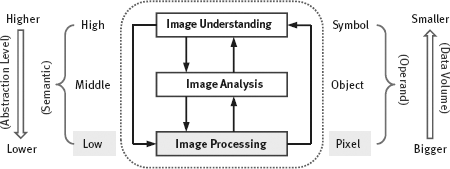
\includegraphics[width=0.8\textwidth, keepaspectratio]{08_Chapter01_fig1-4}
	\caption{\label{fig:sota:imageengineering} Levels of image engineering. 
	Reprinted from \textcite[][Chapter~1]{zhang2017imageprocessing}}
\end{figure}

\subsection{Object Detection}

TODO
edge detection, outline detection
foreground background mask from video image
background substraction

\subsection{Volume Estimation}

TODO
single view, multiview, depth sensors
estimation by pixel area
interpolation of depth information by combinding views
bounding / section box
full 3d reconstruction
\ref{fig:sota:mulitviewtop}

\begin{figure}[hbt]
	\centering
	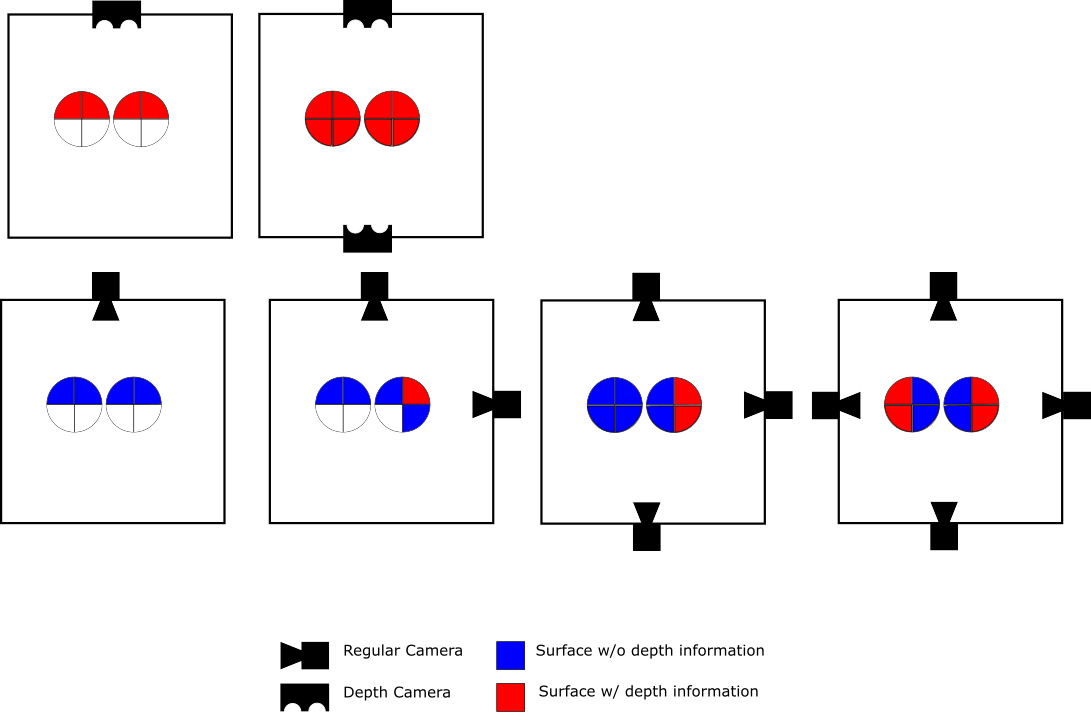
\includegraphics[width=1.0\textwidth, keepaspectratio]{resources/multiview}
	\caption{\label{fig:sota:mulitviewtop}Concept of depth reconstruction in a 2D multi-view situation.
	Based on and adapted from \textcite[][]{sonaten2011volume}}
\end{figure}


\section{Elevator Control}
TODO shor introtuction, definition and what are important aspects about it

\subsection{System Components}

In order to gain an understanding of how an elevator system is controlled,
it is useful to look at the components a general system includes.
To do so, the mechanisms involved in a typical elevator ride 
from a passenger perspective shall be outlined.
Figure \ref{fig:sota:systemcomponents} gives an general overview over the involved logical components and their connections.

\begin{figure}[hbt]
	\centering
	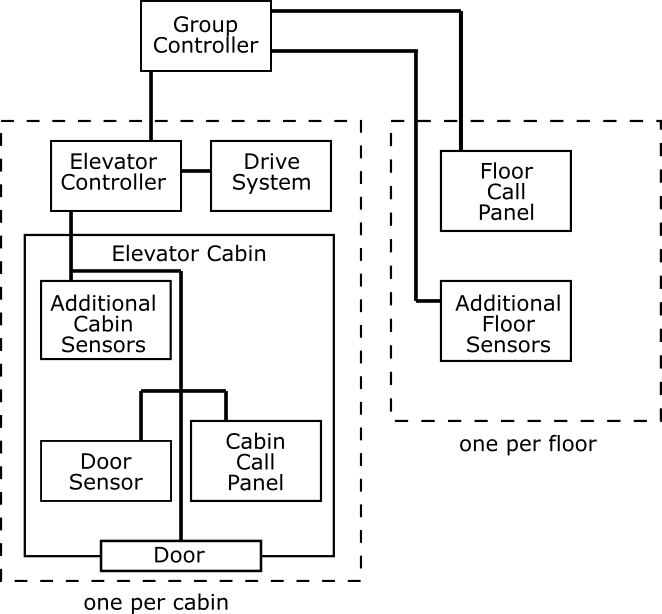
\includegraphics[width=0.8\textwidth, keepaspectratio]{resources/systemcomponets}
	\caption{\label{fig:sota:systemcomponents} General components of an elevator control system. Based on and adapted from \textcite[][pp.~4,16]{xang2016trafficlist},  \textcite[][pp.10]{siikonen1997models}}
\end{figure}

When a passenger wants to take the elevator from one floor to another,
they press a button on the \emph{floor call panel} and issue a \emph{hall call} (or \emph{reservation call}, \emph{landing call}) to the system \autocite[][pp.~6--10]{siikonen1997models}.
This hall call signals to the system that an elevator needs to pick them up.
The button pressed might be a simple push button, but can also be more complex 
and capture information about the direction or destination of travel \autocite[][pp.~89--93]{unger2015aufzuege}.
Even before the passenger presses the panel button, \emph{additional sensors} 
on the floor can detect their intent to use the elevator and gather more information about them.
This can include among others camera systems \autocite[][]{lin2011control}, badge scanners, or \enquote{smart home} installations \autocite[][]{kwon2014sensor}.
In a multi-elevator system the hall call is registered by the \emph{group controller} and stays active until it is deleted when an cabin picks up the passenger.
The group controller \emph{schedules and dispatches} an elevator move to the respective floor and serve the call.
In case of a single-elevator system no group controller is necessary.
Different scheduling algorithms can be used to determine which cabin should serve which hall call next.
The dispatch signal is picked up by the \emph{elevator controller} of the respective cabin, which then instructs the \emph{drive} system to move the elevator along the shaft to the respective floor by actuating the motors.

Once a cabin stops at the floor, it opens its \emph{door} and the passenger enter the elevator.
To select their destination floor, they use the \emph{cabin call panel}.
This \emph{car call} (or \emph{destination call}) \autocite[][pp.~6--10]{siikonen1997models} is passed to the group controller, 
which schedules the elevator to move to the destination floor at some time.
The group controller needs therefore to consider hall calls, as well as car calls in its scheduling algorithm
Before the elevator starts to move, the door closes again, if no obstacle is detected by the \emph{door sensor}.
Until the elevator serves the destination floor, the car call stays active.
\emph{Additional sensors} inside the cabin provide more information about the passengers inside.
This can include among others a weight scale to measure the total weight utilization, or a kind of camera system \autocite[][]{xang2016trafficlist}.
Further more the position of each elevator is known to the group controller.

\subsection{System Classifications}

Elevator systems come in different configurations with different purposes.
Depending on their use cases different technical implementations can chosen.
Therefore they can be classified in various dimensions.

The first observation to make is the \textbf{number of shafts and cabins} in the system.
The main difference comes in the scheduling complexity regarding single-cabin versus multi-cabin systems.
Systems with multiple elevators need a group controller to decide which cabin serves which hall call.
This decision can be non-trivial as laid out in section \vref{sec:sota:strategies}.
When only one cabin is used, the scheduling becomes more straightforward.
In small residential buildings an single cabin might be sufficient.
However in buildings with larger passenger amounts, such as office buildings, a multi-elevator setup can become necessary increase the handling capacity.

Next is the classification by the \textbf{type of objects or people} that are transported in the system. Especially important is the distinction of the purpose of the elevator system regarding whether people and / or large objects can be conveyed.
\textcite[][pp.~141--158]{unger2015aufzuege} describes the properties of the most common types:

\begin{itemize}
    \item Cabins that carry \textbf{only people} 
    typically have a premium interior decoration, such as glass, mirrors or stainless steel.
    Usually also cargo can be transported, but large goods might damage the cabin.
    Examples for a building that uses such elevators are office buildings, residential buildings or hotels.
    
    \item Elevators for \textbf{large cargo and people} 
    have a more simple interior that is more resistant to damage by lifting carts. 
    However security measures regarding the doors are taken, such that the elevator is also safe to use by people. 
    Typically a high payload weight and dimension can be moved.
    Examples for the usage of this type are factories, storage buildings or hospitals. 
    
    \item Lifts that carry \textbf{only small cargo} can be found for example in restaurant kitchens to transport dishes.
    The cabin is not used by people and the system is controlled purely from outside call panels. 
    Due to the size restriction only a smaller weight needs to be transported.
    
    \item Cabins that convey \textbf{only large cargo} but no people can only be controlled from the outside call panel and have fewer safety restrictions, even though the cabin can be entered for loading and unloading. 
\end{itemize}

This excerpt of the list is far from complete and \textcite[][pp.~141--158]{unger2015aufzuege} lists even more types, 
such as lifts for wheel chairs, the never-stopping paternoster or elevators on construction sites.
However these are not in the scope of this thesis and are not further considered.

Another interesting distinction to consider is the \textbf{amount of floors} that is served by an elevator system.
The amount of floors influences the heeded handling capacity of the system.
The more floors there are, the more people need to travel a potentially longer distance.
While a building with only a few floors can be handled by a single elevator,
buildings with up to 40 stories require the use of elevator groups.
When more than 40 floors need to be served, 
introducing a \emph{sky lobby} can be beneficial, 
where a fast shuttle transports passengers between the main lobby and the sky lobby. Passengers can then switch the elevator to reach their final destination \autocite[][p.~9]{hakonen2003simulation}.

%
%TODO
%- by type of sensory to haul the car
%-- single button
%-- direction button
%-- destination control
%-- camera system

%TODO additional travel information: how many people inside and outside, up / down / floor %select inside / outside, everyone presses?, video? 
%destination control system


\subsection{Passenger Traffic Patterns}
Passenger traffic patterns are typical streams of passengers going from one floor to another.
Those patterns are reoccurring regularly based on the time of the day.
The movement of passengers can be described with three directions: \emph{incoming}, \emph{outgoing}, and \emph{inter-floor} traffic.
With those directions the traffic patterns can be described, as they focus on one of the directions, but also incorporates components of passengers heading in other directions \autocite[][p.~259]{siikonen1993simulation}.
According to multiple sources, three general patterns are present in office buildings \autocite[][pp.~1--2]{beers2015arrivals}
\autocite[][pp.~6--7]{axelsson2013strategies}
\autocite[][p.~194]{unger2015aufzuege}
\autocite[][p.~14]{siikonen1997models}:

\begin{itemize}
    \item \textbf{Up-peak traffic} In the morning the majority of passengers in an office building constitutes to an incoming traffic.
    They arrive at the entrance lobby and travel to different upper floors to fill the building.
    The lift cars potentially need to stop at every level and return to the lobby without passengers to pick up new ones. 
    This reduces the utilized capacity and puts a high load on the elevator system to convoy all passengers in time.
    \item \textbf{Down-peak traffic} In the evening the majority of the passengers are leaving the office building and travel from arbitrary upper floors to the main lobby.
    Most of the passengers constitute to outgoing traffic.
    The elevator system needs to pick up passengers at every level. 
    Reverse to the up-peak traffic, the cars are empty when returning from the lobby.
    Similar to the up-peak traffic this situation induces a high stress on the system.
    \item \textbf{Inter-floor traffic} All other traffic that is neither incoming nor outgoing can be considered inter-floor traffic. Passengers that travel from one floor to another but are not entering or leaving the building are the majority in this situation.
\end{itemize}

\begin{figure}[hbt]
	\centering
	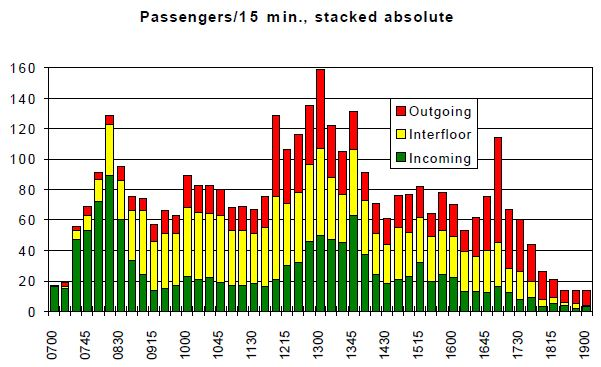
\includegraphics[width=0.8\textwidth, keepaspectratio]{resources/traffictimes}
	\caption{\label{fig:sota:traffictimes} Exemplary traffic component profile for an office building.
	Reprinted from \textcite[][p.~14]{siikonen1997models}}
\end{figure}

%Figure \ref{fig:sota:trafficpatterns} depicts the former mentioned traffic components.
Figure \ref{fig:sota:traffictimes} shows an example of how the traffic components contribute to overall traffic in an office building. A clear peak of incoming traffic in the morning and outgoing traffic in the evening are visible.
This information can be used to model simulations and predict traffic in various circumstances.
It has significant impact on the scheduling principles employed for each situation in order to improve the efficiency of an elevator system.

%\begin{figure}[hbt]
%	\centering
%	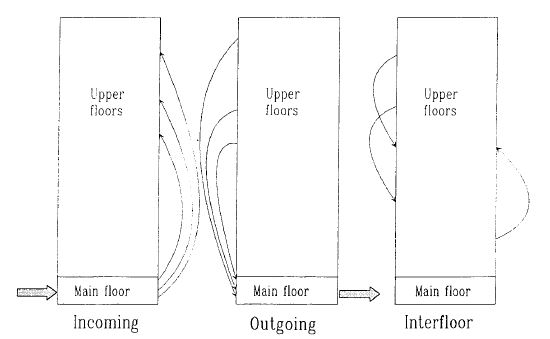
\includegraphics[width=0.8\textwidth, keepaspectratio]{resources/trafficpatterns}
%	\caption[]{\label{fig:sota:trafficpatterns} Typical categories of passenger traffic: Incoming, Outgoing and Inter-floor.
%	Reprinted from \textcite[][p.~259]{siikonen1993simulation}}
%\end{figure}

% TODO or use \textcite[][p.~12]{sorsa2005destination} as broader image 

\subsection{Control Strategies}
\label{sec:sota:strategies}

Elevator control strategies deal with the assignment of hall calls and car calls to elevator rides in order to derive a stopping schedule for the cabins in the system.



TODO
single elevator  vs multi elevator

\autocite[][pp.~3--4,10]{beers2015arrivals}
- stopping policies / strategies
- parking polcies
- call allocation

\autocite[][pp.~3--6]{axelsson2013strategies}
- collective control
- zoneing
- search based
- rule based
- genetic algorithm


- sequential (eg hospital)



\subsection{Performance Criteria}

In order to evaluate the performance of an elevator system some metrics about it are commonly considered.
They are used to check if a planned system fulfills the requirements that the expected traffic poses. 
The metrics are mostly perceived as part of the service quality by the passengers.
Many of them are linked together and influence each other.

% General cite:
%\autocite[][p.~10]{beers2015arrivals}
%\autocite[][p.~7]{hakonen2003simulation}
%\autocite[][pp.8-9]{siikonen1997models}
%\autocite[][p.~194]{unger2015aufzuege}

\begin{itemize}

    \item The \textbf{passenger waiting time} 
        describes the amount of time between the arrival of a passenger at the landing floor 
        and their entry into the elevator cabin 
        \autocite[][p.~7]{hakonen2003simulation}\autocite[][pp.8-9]{siikonen1997models}.
        
    \item The \textbf{passenger ride time} 
        measures the time between the entering of a passenger into the cabin 
        and them exiting the cabin on the destination floor
    \autocite[][pp.8-9]{siikonen1997models}.
    
    \item The \textbf{total journey time}, 
        also called \emph{total service time} \autocite[][p.~10]{beers2015arrivals} or \emph{time to destination},
        describes the total time a passenger spends in the system 
        and is calculated by the sum of waiting and ride time
        \autocite[][pp.8-9]{siikonen1997models}.
        
    \item The \textbf{round trip time} 
        describes the time it takes for a single elevator to collect passengers at the lobby,
        deliver them to the upper floors and return to the lobby. 
        This measure is critical in the up-peak traffic
        \autocite[][pp.8-9]{siikonen1997models}.
        
    \item The \textbf{handling capacity}, 
        also called \emph{5-minute interval}
        \autocite[][p.~194]{unger2015aufzuege},
        describes the maximum number of passengers that can be transported (into the upper most floor) during up-peak traffic
        \autocite[][pp.8-9]{siikonen1997models}.
        It is dependent on the round trip time.
        In theoretical considerations a maximum utilization of 60-80\% of the capacity is used for this scenario
        \autocite[][p.~194]{unger2015aufzuege}\autocite[][p.~7]{hakonen2003simulation}.
    
    \item The \textbf{interval time} 
        describes the time between departures of any cabin from the lobby 
        and influences the time a passenger hat to wait at the lobby
        \autocite[][pp.8-9]{siikonen1997models}.
    
    \item The \textbf{hall call time} 
        describes the time between the issuing of an hall call by a passenger and the cancellation of the call. 
        The call is canceled when an elevator is scheduled to serve the call floor and hence decelerates to stop at the floor
        \autocite[][pp.8-9]{siikonen1997models}. 
    
    \item The number of \textbf{total stops}
        necessary to serve an specified amount of passengers (or within a given time frame) is an indicator for the efficiency of the scheduling algorithm
        \autocite[][p.~194]{unger2015aufzuege}.
    
    \item The \textbf{energy consumption} 
        per ride or per time interval is an measure of economic interest. 
        However it does not influence the perceived service quality.
    
    \item The \textbf{capacity utilization} 
        of the cabins in spacial and weight dimensions is an interesting metric to observe, 
        since usually only 60-80\% of the capacity is used at a time 
        \autocite[][p.~194]{unger2015aufzuege}
        \autocite[][p.~7]{hakonen2003simulation}.
        This utilization can be even lower when large objects are present.
        The average utilization is further influenced by empty rides.
        
\end{itemize}

For each of the metrics it is common to calculate statistical figures, such as average, mean, minimum, maximum and standard deviation, which also can differ depending on the traffic situation.
These calculations can be based on theoretical consideration about the physical parameters of the system \autocite[][p.~194]{unger2015aufzuege}, simulations or heuristical observations in real buildings.
 
When the group controller schedules the elevators in a system, the order of dispatches influences the metrics listed above.
The elevator allocations are calculated by optimization of a cost function which takes the metrics in consideration.
Usually the waiting time is optimized, but also the ride time can be optimized in order to increase the handling capacity. \autocite[][p.~10]{siikonen1997models} 

\subsection{Simulational Optimization Approaches}
TODO
model building etc: here is a lot of research in the topic utilizing theoretical multivariable model optimization, simulational approaches and heuristical approaches in real world (refs?)

\autocite[][pp.~7--11]{beers2015arrivals}
\autocite[][p.~193]{unger2015aufzuege}


TODO
